\chapter{CƠ SỞ LÝ THUYẾT VÀ CÁC CÔNG TRÌNH LIÊN QUAN}
\label{ch:theory}

\section{Mô hình Ngôn ngữ Lớn và Giới hạn trong Suy luận Ký hiệu}
\label{sec:theory_llm}

\subsection{Kiến trúc Transformer và Cơ chế Tự chú ý}
Các mô hình ngôn ngữ lớn (LLM) hiện đại phần lớn được xây dựng trên nền tảng kiến trúc mạng nơ-ron Transformer do Vaswani và các cộng sự giới thiệu năm 2017 \cite{vaswani2017attention}. Trọng tâm của kiến trúc này là cơ chế tự chú ý đa đầu (\textit{Multi-Head Self-Attention}), cho phép mô hình tính toán mức độ phụ thuộc ngữ cảnh giữa mọi cặp token trong chuỗi đầu vào theo phương thức song song, khắc phục điểm nghẽn xử lý tuần tự của các mạng nơ-ron hồi quy (RNN) và mạng bộ nhớ dài-ngắn (LSTM) truyền thống.

Phép tính tự chú ý tích vô hướng có chuẩn hóa được định nghĩa toán học như sau:
\begin{equation}
    \text{Attention}(Q, K, V) = \text{softmax}\left(\frac{Q K^T}{\sqrt{d_k}}\right) V
\end{equation}
Trong đó $Q \in \mathbb{R}^{n \times d_k}$ là ma trận truy vấn, $K \in \mathbb{R}^{m \times d_k}$ là ma trận khóa, $V \in \mathbb{R}^{m \times d_v}$ là ma trận giá trị, và $d_k$ là số chiều của vector khóa dùng làm hệ số chia chuẩn hóa nhằm tránh hiện tượng bão hòa đạo hàm của hàm $\text{softmax}$ khi tích vô hướng có độ lớn cao.

Cơ chế tự chú ý đa đầu mở rộng khả năng biểu diễn bằng cách chiếu các ma trận $Q, K, V$ qua $h$ không gian con tuyến tính độc lập:
\begin{equation}
    \text{MultiHead}(Q, K, V) = \text{Concat}(\text{head}_1, \dots, \text{head}_h) W^O
\end{equation}
với $\text{head}_i = \text{Attention}(Q W_i^Q, K W_i^K, V W_i^V)$, trong đó $W_i^Q, W_i^K, W_i^V$ và $W^O$ là các ma trận trọng số học được trong quá trình huấn luyện.

\subsection{Bản chất Xác suất Tự quy hồi và Hiện tượng Ảo giác}
Khi thực hiện tác vụ tạo sinh văn bản, các LLM như GPT-4 hay Gemma vận hành theo cơ chế giải mã tự quy hồi. Tại mỗi bước thời gian $t$, mô hình tính toán phân phối xác suất trên toàn bộ từ vựng $\mathcal{V}$ để lấy mẫu token kế tiếp:
\begin{equation}
    w_t \sim P(w_t \mid w_1, w_2, \dots, w_{t-1}; \Theta) = \text{softmax}\left( \frac{z_t}{\tau} \right)
\end{equation}
trong đó $z_t$ là vector logit đầu ra của Transformer, $\tau$ là tham số nhiệt độ điều chỉnh mức độ ngẫu nhiên, và $\Theta$ là tập trọng số của mô hình.

Hàm mục tiêu huấn luyện dựa trên nguyên lý cực đại hóa hàm hợp lý (\textit{Maximum Likelihood Estimation}) trên tập ngữ liệu:
\begin{equation}
    \mathcal{L}(\Theta) = - \sum_{i=1}^N \log P(w_i \mid w_{<i}; \Theta)
\end{equation}

Hệ quả trực tiếp là LLM tối ưu hóa độ trôi chảy thống kê của chuỗi từ chứ không bảo đảm tính đúng đắn của các mệnh đề logic hình thức. Hiện tượng ảo giác thông tin thường xuất hiện từ ba nguyên nhân:
\begin{enumerate}[leftmargin=1.5cm]
    \item \textbf{Thiếu bộ nhớ trạng thái thế giới có ràng buộc:} Mô hình không duy trì một cấu trúc dữ liệu tường minh để khóa chặt vị trí vật lý, mốc thời gian và quan hệ sở hữu giữa các thực thể.
    \item \textbf{Suy giảm chú ý theo chiều dài ngữ cảnh:} Khi hồ sơ vụ án kéo dài qua nhiều đoạn văn, phân phối chú ý dễ bị phân tán, dẫn tới việc mô hình bỏ sót ràng buộc đã thiết lập ở phần đầu.
    \item \textbf{Lan truyền sai số suy luận:} Trong chuỗi suy luận nhiều bước, một sai lệch nhỏ ở bước trung gian sẽ điều kiện hóa toàn bộ các token sinh ra tiếp theo, gây mất nhất quán dây chuyền.
\end{enumerate}

\subsection{Giới hạn của Các Kỹ thuật Kích thích Suy luận Đơn thuần}
Các kỹ thuật hướng dẫn câu lệnh như suy luận theo chuỗi (CoT) \cite{wei2022chain} hay cây suy nghĩ (\textit{Tree-of-Thoughts}) yêu cầu mô hình tự diễn giải từng bước trung gian trước khi kết luận. Tuy nhiên, các nghiên cứu thực nghiệm chỉ ra rằng CoT vẫn gặp khó khăn khi duy trì tính nhất quán của hệ ràng buộc đóng trên văn bản dài \cite{sprague2024musr, li2024contradoc}. Khi biên soạn một vụ án mạng, LLM có thể viết ra chuỗi lập luận CoT mạch lạc về mặt ngôn từ nhưng vẫn vi phạm tính toán thời gian hoặc gán nhầm mã định danh nhân vật. Vì vậy, việc tách khâu kiểm định logic khỏi cơ chế sinh xác suất của LLM là cần thiết.

\section{Phương pháp Tiếp cận Trí tuệ Nhân tạo Neuro-Symbolic}
\label{sec:theory_neurosymbolic}

\subsection{Lý thuyết Quá trình Kép và Phân loại Kiến trúc Kautz}
Trong tâm lý học nhận thức, Daniel Kahneman đề xuất Lý thuyết Quá trình Kép (\textit{Dual-Process Theory}) \cite{kahneman2011thinking}, phân biệt hai phương thức xử lý thông tin: Hệ thống 1 (\textit{System 1}) trực giác, phản ứng nhanh và Hệ thống 2 (\textit{System 2}) logic, thận trọng:
\begin{itemize}[leftmargin=1.5cm]
    \item \textbf{Hệ thống 1 (Nhanh, Trực giác):} Xử lý tự động các tác vụ nhận dạng mẫu hình, liên tưởng ngữ nghĩa và tạo sinh ngôn ngữ tự nhiên.
    \item \textbf{Hệ thống 2 (Chậm, Phân tích):} Đòi hỏi kiểm chứng có hệ thống, vận hành trên quy tắc hình thức, tính toán số học và đối chiếu giả thuyết.
\end{itemize}

Giáo sư Henry Kautz \cite{kautz2022third} phân loại các hệ thống AI lai Neuro-Symbolic thành 6 nhóm kiến trúc chính:
\begin{enumerate}[leftmargin=1.5cm]
    \item \textit{Type 1 (Symbolic[Neuro]):} Đầu vào ký hiệu được ánh xạ vào không gian vector nơ-ron (như mô hình biểu diễn ngôn ngữ hai chiều BERT).
    \item \textit{Type 2 ([Neuro]Symbolic):} Mạng nơ-ron trích xuất đặc trưng cảm biến ở tầng dưới để cấp cho bộ suy luận ký hiệu ở tầng trên.
    \item \textit{Type 3 (Neuro; Symbolic):} Thành phần nơ-ron đề xuất giả thuyết (Hệ thống 1), sau đó được kiểm chứng và phản hồi bởi động cơ ký hiệu độc lập (Hệ thống 2) trong vòng lặp đóng.
    \item \textit{Type 4 (Neuro:Symbolic $\to$ Neuro):} Tri thức ký hiệu được biên dịch thành thành phần hàm mất mát khả vi để huấn luyện mạng nơ-ron.
    \item \textit{Type 5 (Neuro\_Symbolic):} Cấu trúc biểu diễn ký hiệu được nhúng trực tiếp vào kiến trúc nơ-ron.
    \item \textit{Type 6 (Embodied / Deep Reasoning):} Mô hình tự học và trừu tượng hóa quy tắc ký hiệu thông qua tương tác với môi trường.
\end{enumerate}

Kiến trúc trong đồ án kế thừa mô hình \textbf{Type 3 (Neuro; Symbolic)} kết hợp góc nhìn dung hợp của Garnelo và Shanahan \cite{garnelo2019reconciling}:
\begin{itemize}[leftmargin=1.5cm]
    \item \textbf{Thành phần Nơ-ron:} Đảm nhiệm vai trò Hệ thống 1, tận dụng năng lực sáng tạo văn cảnh, động cơ tâm lý, lời khai và mô tả hiện trường của LLM.
    \item \textbf{Thành phần Ký hiệu:} Đảm nhiệm vai trò Hệ thống 2, vận hành như màng lọc tất định kiểm tra các bất biến về nhiệt học thi thể, tính toàn vẹn định danh và quan hệ đồ thị.
\end{itemize}

\subsection{Mô hình Tương tác Vòng lặp Kín trong Sinh Kịch bản}
Luồng phối hợp giữa hai thành phần trong đồ án được tổ chức qua ba pha tuần tự có phản hồi:
\begin{enumerate}[leftmargin=1.5cm]
    \item \textbf{Pha Tạo sinh:} Chuỗi tác tử LLM đề xuất cốt truyện, thông số pháp y, lời khai nghi phạm và vật chứng dưới dạng dữ liệu có cấu trúc.
    \item \textbf{Pha Thẩm định Ký hiệu:} Bộ kiểm định tất định tính toán lại cửa sổ tử vong theo mô hình Henssge và đối chiếu toàn bộ ràng buộc trên tập nghi phạm -- chứng cứ.
    \item \textbf{Pha Phản hồi Định hướng:} Khi phát hiện vi phạm, bộ kiểm định xuất tín hiệu chẩn đoán có cấu trúc (gồm mã loại lỗi, phân hệ chịu trách nhiệm và mô tả chi tiết) để hướng dẫn tác tử tương ứng sửa lỗi cục bộ.
\end{enumerate}

\section{Giải tích Nhiệt học Pháp y: Mô hình Hai hàm mũ Henssge}
\label{sec:theory_henssge}

\subsection{Cơ sở Sinh học và Bộ ba Dấu hiệu Tử thi}
Trong y pháp hình sự, việc ước lượng khoảng thời gian sau tử vong (PMI) dựa trên ba biến đổi sinh lý kinh điển \cite{madea2005recent}:
\begin{enumerate}[leftmargin=1.5cm]
    \item \textbf{Sự làm lạnh thi thể (\textit{algor mortis}):} Quá trình tỏa nhiệt thụ động sau khi quá trình trao đổi chất chấm dứt, đưa thân nhiệt tiệm cận nhiệt độ môi trường.
    \item \textbf{Sự co cứng cơ tử thi (\textit{rigor mortis}):} Hiện tượng co cứng sợi cơ do cạn kiệt nguồn năng lượng phân tử ATP sau chết, thường khởi phát sau 2--4 giờ và đạt cực đại quanh 12 giờ.
    \item \textbf{Sự hoen ố tử thi (\textit{livor mortis}):} Sự lắng đọng hồng cầu theo trọng lực tại vùng thấp của cơ thể, dần cố định màu sắc sau 6--8 giờ.
\end{enumerate}

Trong ba dấu hiệu nêu trên, tốc độ hạ thân nhiệt trực tràng là đại lượng phù hợp nhất để mô hình hóa định lượng trong 24--48 giờ đầu tiên.

\subsection{Hạn chế của Mô hình Làm lạnh Newton Tuyến tính}
Nếu áp dụng đơn thuần định luật làm lạnh của Newton:
\begin{equation}
    \frac{dT}{dt} = -k (T - T_{\text{ambient}}) \implies T(t) = T_{\text{ambient}} + (T_0 - T_{\text{ambient}}) e^{-kt}
\end{equation}
mô hình sẽ không phản ánh được giai đoạn 2--3 giờ đầu sau tử vong, khi lõi cơ thể vẫn duy trì \textbf{bình nguyên nhiệt độ} với tốc độ giảm nhiệt ban đầu gần bằng 0 ($dT/dt \approx 0$). Sai lệch này có thể làm lệch ước tính PMI nhiều giờ, gây mâu thuẫn với khung giờ ngoại phạm trong kịch bản trinh thám.

\subsection{Phương trình Hai hàm mũ Henssge}
Năm 1988, Claus Henssge công bố mô hình chuẩn hóa hai hàm mũ giải quyết hiệu ứng bình nguyên nhiệt học \cite{henssge1988death, henssge2000estimation}. Tỷ lệ hạ nhiệt chuẩn hóa $\Phi(t)$ tại thời điểm $t$ (giờ) sau tử vong được xác định theo hai ngưỡng nhiệt độ môi trường $T_{\text{ambient}}$:
\begin{equation}
    \Phi(t) = \frac{T_{\text{body}} - T_{\text{ambient}}}{37.2 - T_{\text{ambient}}} =
    \begin{cases}
        1.25 \cdot e^{-k t} - 0.25 \cdot e^{-5k t}, & \text{nếu } T_{\text{ambient}} \le 23.2^\circ\text{C} \\
        1.11 \cdot e^{-k t} - 0.11 \cdot e^{-10k t}, & \text{nếu } T_{\text{ambient}} > 23.2^\circ\text{C}
    \end{cases}
    \label{eq:henssge_formula}
\end{equation}
Trong phương trình (\ref{eq:henssge_formula}):
\begin{itemize}[leftmargin=1.5cm]
    \item $T_{\text{body}}$ là thân nhiệt trực tràng đo được tại thời điểm phát hiện thi thể ($^\circ\text{C}$);
    \item $T_{\text{ambient}}$ là nhiệt độ môi trường nơi phát hiện thi thể ($^\circ\text{C}$);
    \item $37.2^\circ\text{C}$ là giá trị thân nhiệt trực tràng chuẩn lúc tử vong;
    \item Số hạng âm thứ hai giúp triệt tiêu đạo hàm tại $t=0$, tái hiện chính xác giai đoạn bình nguyên nhiệt học ban đầu.
\end{itemize}

Hệ số truyền nhiệt $k$ (đơn vị $\text{giờ}^{-1}$) phụ thuộc phi tuyến vào khối lượng cơ thể nạn nhân $M$ (kg) và hệ số hiệu chỉnh trang phục/môi trường $C$:
\begin{equation}
    k = \frac{1.2815}{(M \cdot C)^{0.625}} - 0.0284
    \label{eq:henssge_k}
\end{equation}
Các giá trị điển hình của $C$ theo quy chuẩn y pháp: $C = 1.0$ (quần áo mỏng trong không khí tĩnh), $C = 1.1\text{--}1.2$ (áo ấm hoặc đắp chăn), $C = 0.75\text{--}0.9$ (ít trang phục hoặc nơi thoáng gió) và $C = 0.5$ (trong nước tĩnh).

\begin{figure}[H]
    \centering
    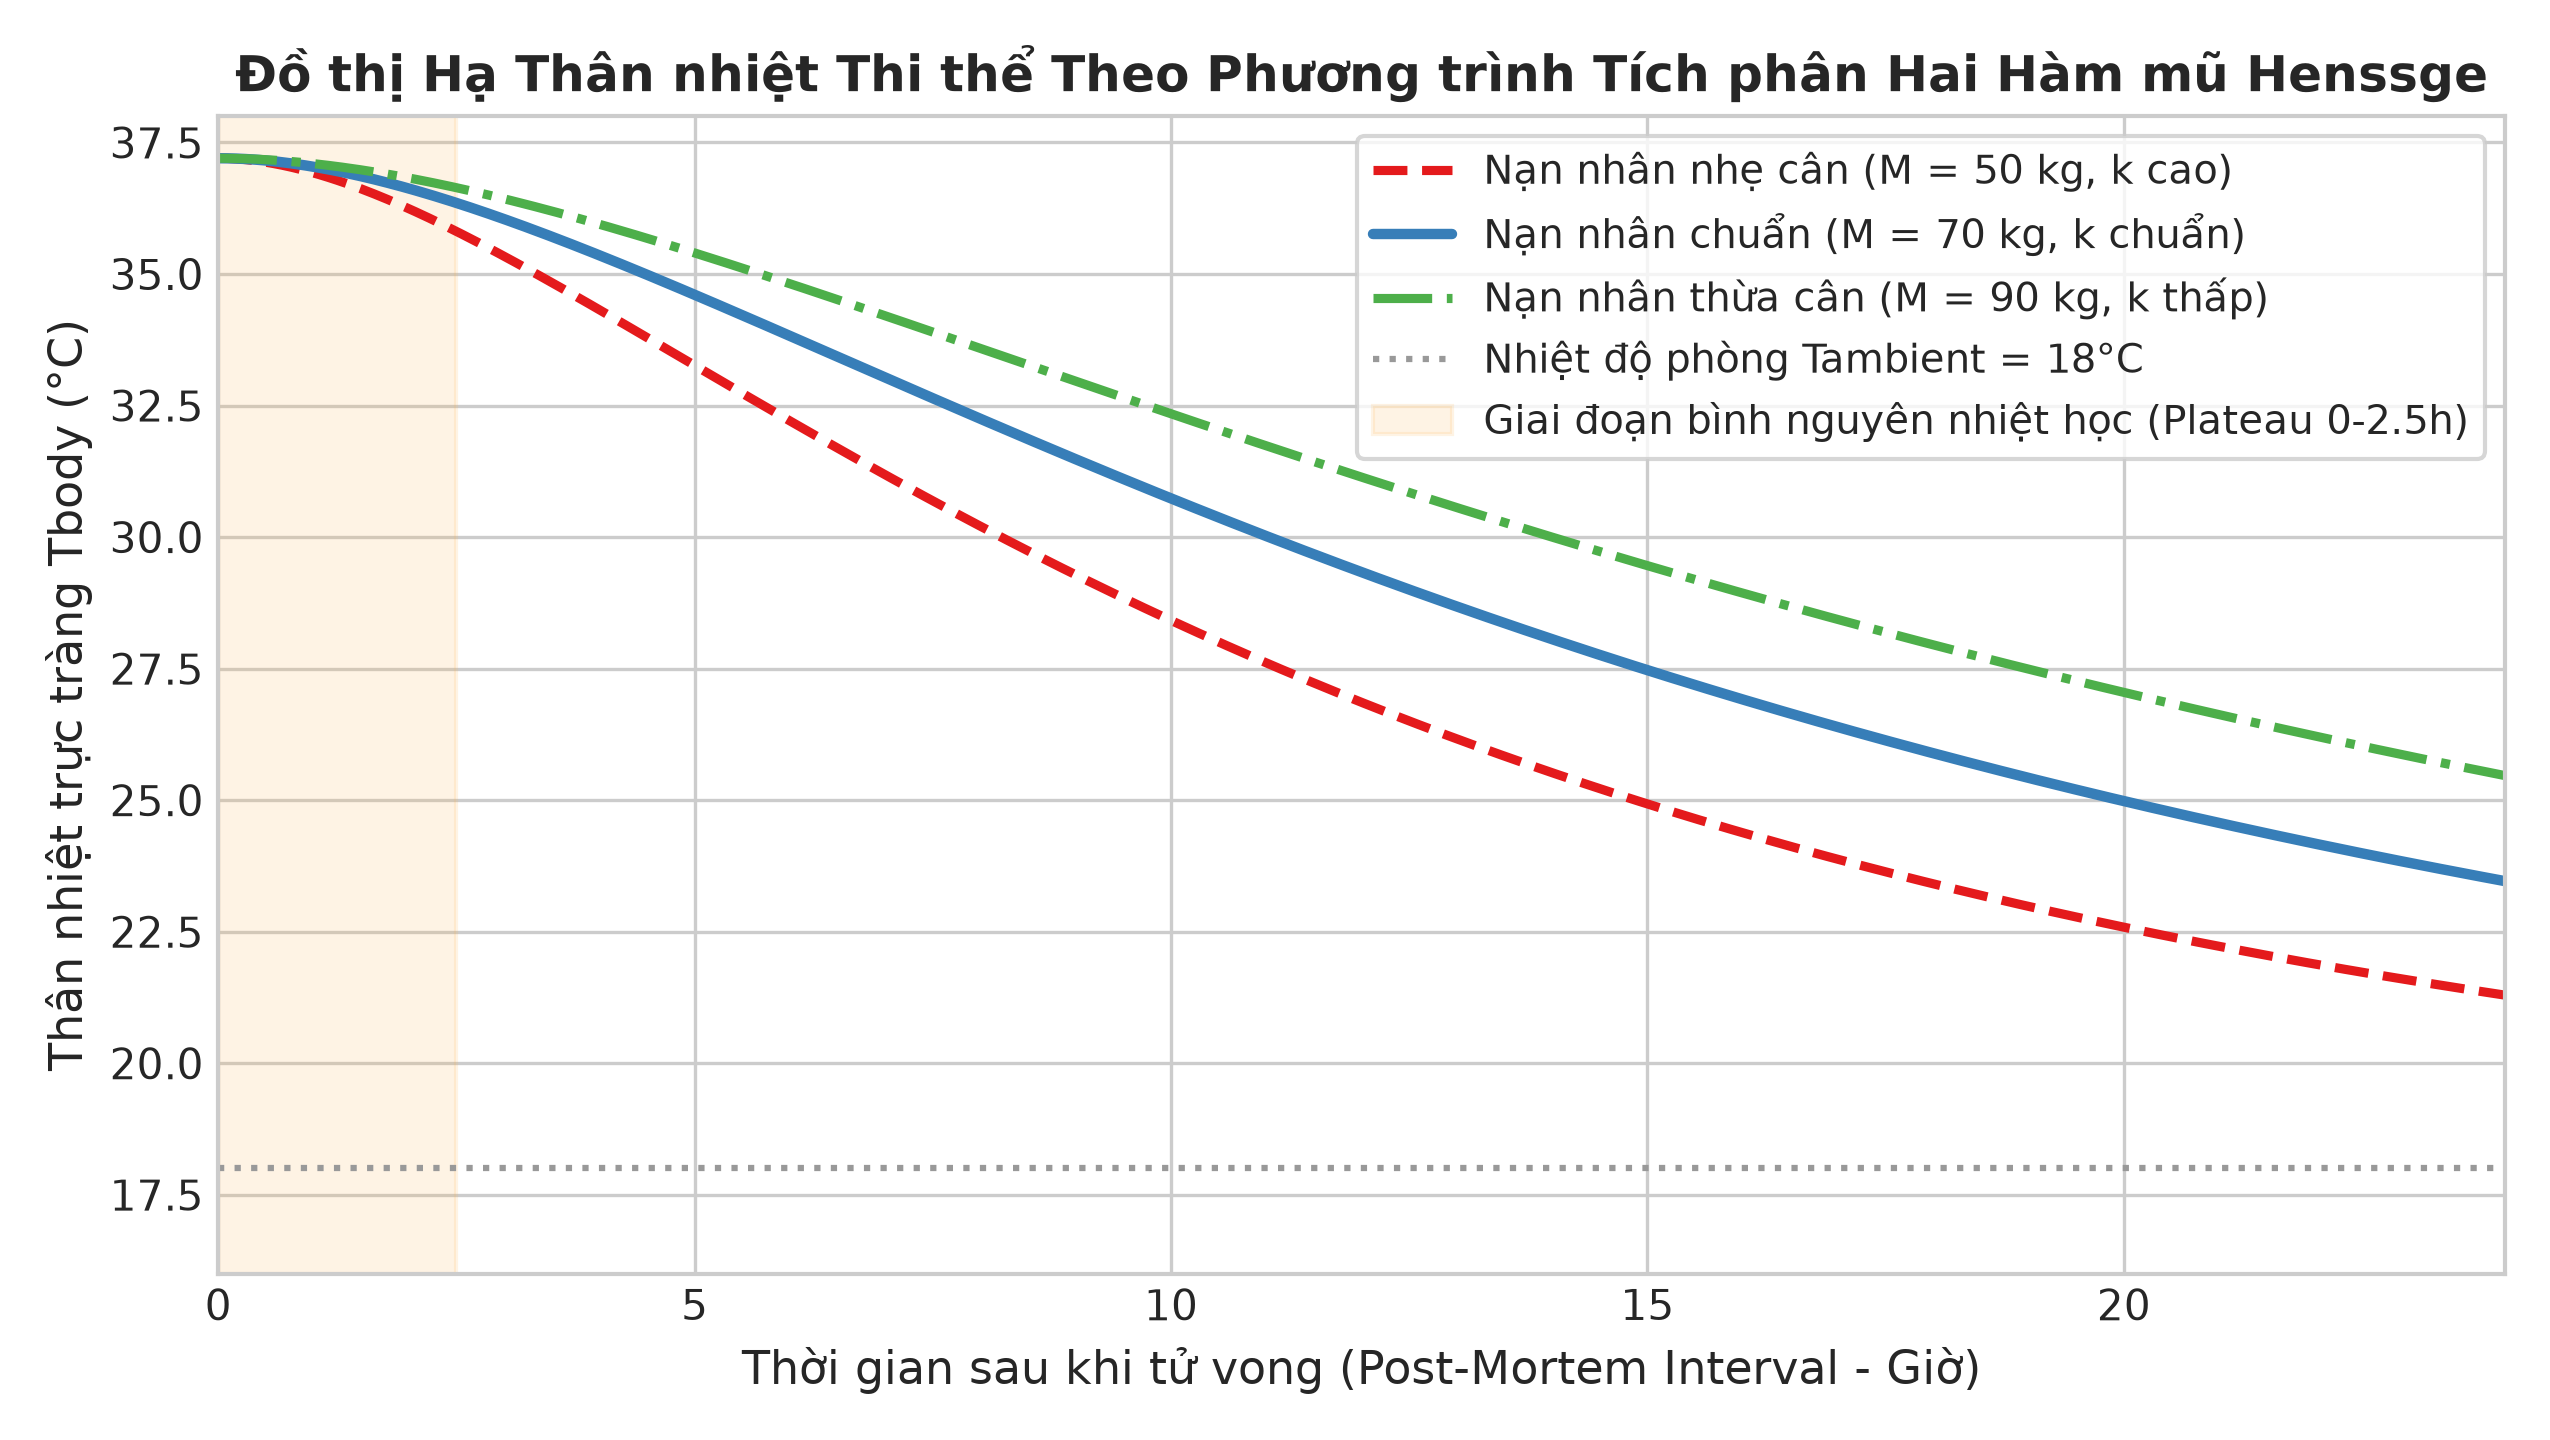
\includegraphics[width=0.85\textwidth]{henssge_curves.png}
    \caption{Đồ thị Hạ thân nhiệt Thi thể Theo Phương trình Hai Hàm mũ Henssge với Các Mức Khối lượng Khác nhau ($T_{\text{ambient}} = 18^\circ\text{C}$)}
    \label{fig:henssge_curves}
\end{figure}

\subsection{Thuật toán Chia đôi Tìm Nghiệm Số và Cửa sổ Tử vong TOD}
Vì phương trình (\ref{eq:henssge_formula}) là phương trình siêu việt đối với $t$ nhưng hàm $\Phi(t)$ đơn điệu giảm ngặt trên $[0, 48]$ giờ từ giá trị $\Phi(0) = 1$, hệ thống sử dụng phương pháp chia đôi (\textit{bisection method}) trên miền $[0, 48]$ giờ với sai số hội tụ $\epsilon = 10^{-4}$ và tối đa $N_{\text{max}} = 100$ bước lặp để tìm nghiệm duy nhất $t^*$ (Thuật toán \ref{alg:henssge_bisection}).

\begin{algorithm}[H]
\caption{Tìm Nghiệm Thời gian Tử vong Henssge Bằng Phương pháp Chia đôi}
\label{alg:henssge_bisection}
\begin{algorithmic}[1]
\Require $T_{\text{body}}$, $T_{\text{ambient}}$, $M$, $C$, Sai số $\epsilon = 10^{-4}$, Số bước tối đa $N_{\text{max}} = 100$
\Ensure Thời gian sau tử vong $t^*$ (giờ) hoặc $\text{None}$ nếu phi vật lý
\State $k \gets \frac{1.2815}{(M \cdot C)^{0.625}} - 0.0284$
\State $\Phi_{\text{target}} \gets \frac{T_{\text{body}} - T_{\text{ambient}}}{37.2 - T_{\text{ambient}}}$
\If{$\Phi_{\text{target}} \le 0$} \Return $\text{None}$ \EndIf
\If{$\Phi_{\text{target}} \ge 1$} \Return $0.0$ \EndIf
\State Định nghĩa $\Phi(t)$ theo (\ref{eq:henssge_formula}) ứng với ngưỡng $T_{\text{ambient}} \le 23.2^\circ\text{C}$ hoặc $> 23.2^\circ\text{C}$
\State $a \gets 0.0, \; b \gets 48.0$ \Comment{Biên tìm kiếm từ 0 đến 48 giờ}
\If{$\Phi(b) - \Phi_{\text{target}} > 0$} \Return $\text{None}$ \EndIf
\For{$n = 1$ \textbf{to} $N_{\text{max}}$}
    \State $m \gets (a + b) / 2$
    \State $f(m) \gets \Phi(m) - \Phi_{\text{target}}$
    \If{$|f(m)| < \epsilon$ \textbf{or} $(b - a) / 2 < \epsilon$}
        \State \Return $m$
    \ElsIf{$(\Phi(a) - \Phi_{\text{target}}) \cdot f(m) < 0$}
        \State $b \gets m$
    \Else
        \State $a \gets m$
    \EndIf
\EndFor
\State \Return $(a + b) / 2$
\end{algorithmic}
\end{algorithm}

Với dung sai tin cậy tiêu chuẩn $\Delta t = \pm 1.5$ giờ từ thời điểm phát hiện thi thể $T_{\text{discovery}}$, cửa sổ thời gian tử vong (TOD) được động cơ ký hiệu tính trực tiếp và gán khóa cứng cho hồ sơ:
\begin{equation}
    TOD = \left[ T_{\text{discovery}} - (t^* + 1.5), \; T_{\text{discovery}} - \max(0, t^* - 1.5) \right]
\end{equation}

Mọi hồ sơ hợp lệ phải thỏa mãn ràng buộc vật lý:
\begin{equation}
    T_{\text{actual\_crime\_time}} \in TOD
\end{equation}

\section{Biểu diễn Đồ thị Hai phía và Ràng buộc Giải được của Vụ án}
\label{sec:theory_graph}

\subsection{Mô hình hóa Vụ án Dưới dạng Đồ thị Hai phía}
Để kiểm tra cấu trúc suy luận giữa lời khai và vật chứng một cách tường minh, hồ sơ vụ án được ánh xạ sang một đồ thị hai phía có hướng:
\begin{equation}
    G = (V_N \cup V_P, E_R)
\end{equation}
Trong đó:
\begin{itemize}[leftmargin=1.5cm]
    \item Phân hoạch thứ nhất $V_N$ biểu diễn tầng tường thuật gồm các đỉnh nghi phạm $V_S = \{s_1, \dots, s_n\}$ và các đỉnh lời khai ngoại phạm tương ứng;
    \item Phân hoạch thứ hai $V_P$ biểu diễn tầng thực tế hiện trường gồm các đỉnh chứng cứ $V_E = \{e_1, \dots, e_m\}$ và mốc sự kiện thời gian gây án;
    \item Tập cạnh $E_R$ biểu diễn các quan hệ ngữ nghĩa đã gán nhãn giữa hai phân hoạch.
\end{itemize}

\begin{figure}[H]
    \centering
    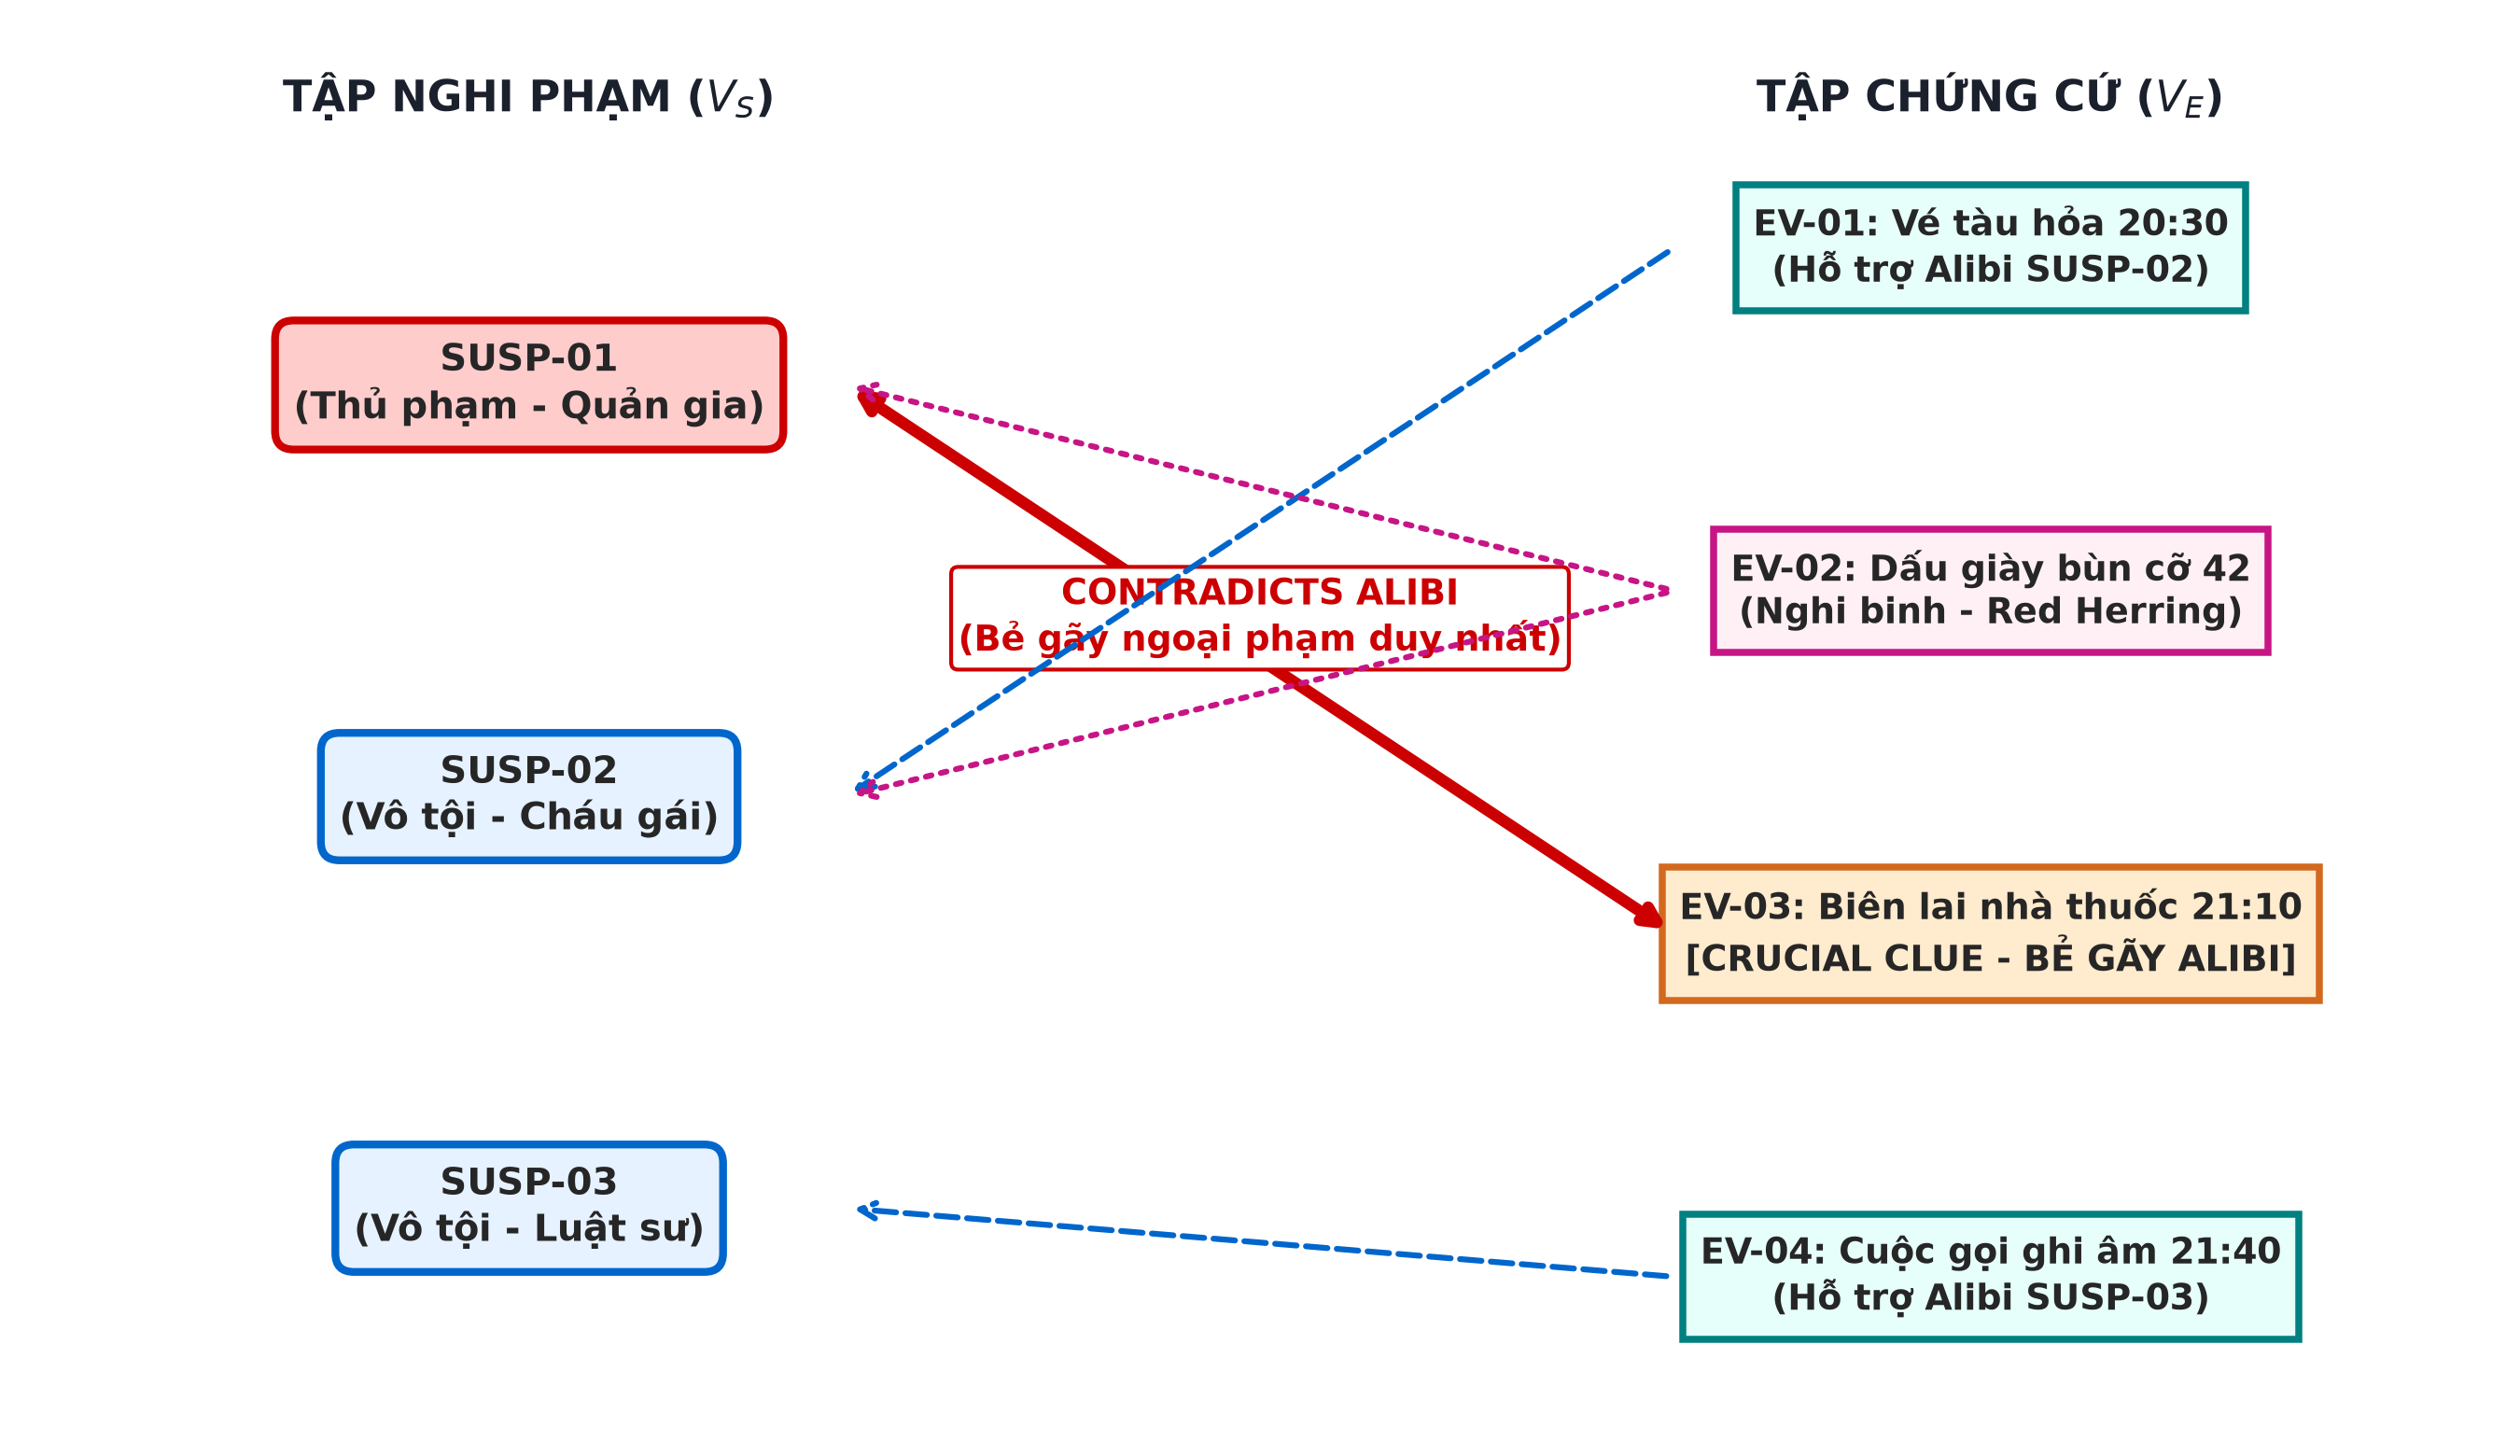
\includegraphics[width=0.90\textwidth]{bipartite_graph.png}
    \caption{Mô hình Đồ thị Hai phía Minh họa Quan hệ Giữa Tập Nghi phạm ($V_S$) và Tập Chứng cứ ($V_E$)}
    \label{fig:bipartite_graph_diagram}
\end{figure}

Các cạnh liên kết trong đồ thị được phân loại thành ba nhóm quan hệ chính:
\begin{enumerate}[leftmargin=1.5cm]
    \item \textbf{Cạnh Tuyên bố / Xác nhận Ngoại phạm:} Liên kết giữa nghi phạm và khung giờ ngoại phạm hoặc chứng cứ hỗ trợ người vô tội.
    \item \textbf{Cạnh Bẻ gãy Ngoại phạm ($E_{\text{contradict}}$):} Liên kết từ vật chứng then chốt (\texttt{is\_crucial = True}) bác bỏ trực tiếp lời khai ngoại phạm của hung thủ.
    \item \textbf{Cạnh manh mối nghi binh (\textit{red herring})} ($E_{\text{herring}}$): Liên kết từ manh mối đánh lạc hướng (\texttt{is\_red\_herring = True}) tới nghi phạm vô tội nhằm giữ độ khó suy luận cho trò chơi.
\end{enumerate}

\subsection{Các Bất biến Thiết kế Bảo đảm Tính Giải được Độc nhất}

\begin{definition}[Khung giờ Ngoại phạm Bao trùm]
Một nghi phạm $s$ có lời khai ngoại phạm che phủ thời điểm phạm tội nếu khoảng thời gian tự khai $[s.\text{alibi\_start}, s.\text{alibi\_end}]$ chứa mốc $T_{\text{actual\_crime\_time}}$ trong cửa sổ $TOD$ (xử lý được cả trường hợp khung giờ vắt qua nửa đêm).
\end{definition}

\begin{invariant}[Hệ Ràng buộc Tính Giải được và Công bằng]
Một hồ sơ vụ án đạt chuẩn kiểm định cấu trúc và giải được công bằng khi tập thực thể và đồ thị $G$ thỏa mãn đồng thời bốn điều kiện tất định sau:
\begin{enumerate}[label=(\roman*)]
    \item \textbf{Tính duy nhất của thủ phạm:} Tồn tại duy nhất một nghi phạm $s^* \in V_S$ được đánh dấu \texttt{is\_culprit = True}, đồng thời định danh của $s^*$ khớp với trường chân lý gốc:
    \begin{equation}
        |\{s \in V_S \mid s.\text{is\_culprit} = \text{True}\}| = 1 \quad \land \quad s^*.\text{id} = \text{GroundTruth.culprit\_id}
    \end{equation}
    
    \item \textbf{Tính tồn tại của chứng cứ phá vỡ ngoại phạm:} Tập vật chứng chứa ít nhất một manh mối then chốt ($\mathcal{C}_{\text{crucial}} = \{e \in V_E \mid e.\text{is\_crucial} = \text{True}\} \neq \emptyset$), bảo đảm nếu thủ phạm có lời khai che phủ thời điểm gây án thì tồn tại đường nối bác bỏ ngoại phạm trên đồ thị.
    
    \item \textbf{Tính toàn vẹn tham chiếu thực thể:} Mọi mã định danh nghi phạm được liên kết bởi các vật chứng hoặc các bước suy luận phải thuộc tập đỉnh hiện hữu $V_S$:
    \begin{equation}
        \forall e \in V_E, \; (e.\text{linked\_suspect\_id} \neq \text{None}) \implies e.\text{linked\_suspect\_id} \in \{s.\text{id} \mid s \in V_S\}
    \end{equation}
    
    \item \textbf{Tính cân bằng yếu tố nghi binh (theo cấu hình sinh án):} Để hạn chế tình huống người chơi đoán đúng chỉ bằng phép loại trừ đơn giản, \texttt{ClueAgent} và bộ kiểm định chất lượng hậu kiểm khuyến nghị bổ sung ít nhất một manh mối đánh lạc hướng gắn với nghi phạm vô tội có bí mật riêng.
\end{enumerate}
\end{invariant}

Trong phần mềm thực tế (\texttt{validator.py} và \texttt{case\_graph.py}), các điều kiện (i), (ii), (iii) cùng ràng buộc nhiệt học Henssge được kiểm tra tất định bằng các phép kiểm tra điều kiện, phép giao tập hợp và duyệt chỉ mục trước khi lưu hồ sơ vào cơ sở dữ liệu.

\section{Hình thức hóa Nguyên tắc Trinh thám Công bằng Knox}
\label{sec:theory_knox}

Bảng \ref{tab:knox_formalization} đối chiếu việc ánh xạ các quy tắc kinh điển trong Mười điều răn của Ronald Knox (1929) \cite{knox1929ten} sang các ràng buộc kỹ thuật được cài đặt trong mã nguồn hệ thống:

\begin{table}[H]
\centering
\caption{Ánh xạ Các Quy tắc Trinh thám Knox sang Ràng buộc Hệ thống}
\label{tab:knox_formalization}
\begin{tabularx}{\textwidth}{p{1.4cm} p{6.2cm} X}
\toprule
\textbf{Điều} & \textbf{Quy tắc Văn học Knox (1929)} & \textbf{Ràng buộc Hệ thống Tương ứng} \\
\midrule
\textbf{Điều 1} & Không có yếu tố siêu nhiên hay ma quái can thiệp vào vụ án. & Thời điểm tử vong và hạ thân nhiệt phải thỏa mãn phương trình nhiệt học Henssge. \\
\textbf{Điều 2} & Không dùng các chất độc giả tưởng chưa được khoa học biết đến. & Vũ khí và nguyên nhân tử vong phải là vật thể hoặc cơ chế vật lý có thật. \\
\textbf{Điều 3} & Không giấu lối đi bí mật chưa từng được mô tả trước. & Toàn bộ địa điểm hiện trường và vị trí thu giữ vật chứng được công bố trong hồ sơ. \\
\textbf{Điều 4} & Thủ phạm phải xuất hiện từ đầu, không thêm nhân vật lúc kết thúc. & Toàn bộ nghi phạm cố định trong $V_S$; ràng buộc \texttt{culprit\_id} phải thuộc tập $\{s.\text{id}\}$. \\
\textbf{Điều 5} & Thám tử điều tra không được tự mình là hung thủ. & Vai trò người chơi tách biệt hoàn toàn với danh sách nghi phạm $V_S$. \\
\textbf{Điều 6} & Không phá án nhờ trực giác hay trùng hợp ngẫu nhiên. & Hàm chấm điểm yêu cầu chọn đúng $s^*$ đồng thời nộp ít nhất một vật chứng thuộc $\mathcal{C}_{\text{crucial}}$. \\
\textbf{Điều 7} & Không dùng anh chị em sinh đôi chưa báo trước làm ngoại phạm giả. & Kiểm tra trùng lặp mã định danh trên toàn bộ tập nghi phạm và vật chứng. \\
\textbf{Điều 8} & Không giấu giếm người chơi các manh mối quan trọng. & Toàn bộ các vật chứng trong $V_E$ đều được truyền và hiển thị trên bảng điều tra. \\
\bottomrule
\end{tabularx}
\end{table}

\section{Khảo cứu và Phân tích Đối chiếu Các Công trình Liên quan}
\label{sec:theory_related_works}

Việc ứng dụng AI vào đánh giá suy luận và tạo sinh tự sự trinh thám đã nhận được sự quan tâm rộng rãi từ cộng đồng xử lý ngôn ngữ tự nhiên. Dưới đây là phân tích đối chiếu ba công trình tiêu biểu công bố trên các hội nghị khoa học uy tín:

\subsection{Bộ đánh giá Suy luận MuSR (Sprague và cộng sự, ICLR 2024)}
Công trình \textit{MuSR} của nhóm nghiên cứu Đại học Texas tại Austin \cite{sprague2024musr} xây dựng bộ dữ liệu đánh giá khả năng suy luận nhiều bước trên văn bản tự sự tự nhiên, trong đó trọng tâm là tập kịch bản án mạng bí ẩn dài khoảng 1,000 từ. MuSR áp dụng quy trình tổng hợp neuro-symbolic từ cây suy luận sang văn bản nhằm tạo bài toán kiểm tra năng lực CoT của GPT-4 và các mô hình tương đương. Kết quả cho thấy ngay cả các mô hình mạnh vẫn gặp sai sót khi theo dõi nhiều mối quan hệ phụ thuộc dài. Tuy nhiên, MuSR được thiết kế như một \textbf{bộ benchmark đánh giá thụ động}, không phải một hệ thống trò chơi tương tác thời gian thực, không tích hợp mô hình nhiệt học y pháp Henssge và không hỗ trợ cơ chế vá lỗi cục bộ theo phản hồi kiểm định.

\subsection{Khung Đa tác tử Deciphering Digital Detectives (Wu và cộng sự, ACL 2024)}
Công trình \textit{Deciphering Digital Detectives} \cite{wu2024deciphering} nghiên cứu hành vi của các tác tử LLM khi tham gia trò chơi nhập vai trinh thám kịch bản \textit{Jubensha} (dạng kịch bản án mạng nhiều người chơi phổ biến). Các tác giả xây dựng bộ dữ liệu từ kịch bản có sẵn và tổ chức hệ đa tác tử đóng vai nghi phạm, trao đổi thông tin, che giấu động cơ và suy luận tìm hung thủ dưới sự hỗ trợ của máy trạng thái hữu hạn (FSM) hoặc prompt điều phối. Dù làm rõ được hành vi tương tác xã hội của LLM, công trình này tập trung vào việc cho tác tử \textit{chơi trên kịch bản đã soạn sẵn bởi con người}, chưa giải quyết bài toán tự động tạo sinh vụ án mới có kiểm chứng tính giải được bằng đồ thị và ràng buộc vật lý.

\subsection{Hệ thống Phát hiện Tự mâu thuẫn ContraDoc (Li và cộng sự, NAACL 2024)}
Công trình \textit{ContraDoc} \cite{li2024contradoc} đề xuất tập dữ liệu gán nhãn thủ công nhằm đo lường khả năng phát hiện các mâu thuẫn tự thân bên trong văn bản dài của các LLM. Nghiên cứu chứng minh LLM dễ bỏ sót các xung đột logic ngầm định nằm cách xa nhau theo dòng thời gian hoặc trạng thái sự kiện. Tương tự MuSR, ContraDoc đóng vai trò là bài toán \textbf{phân loại và phát hiện lỗi hậu kiểm trên văn bản tổng quát}, chưa tích hợp vào vòng lặp sinh kịch bản trò chơi có kiến trúc sửa lỗi cục bộ và chấm điểm suy luận người chơi.

\subsection{Bảng Tổng hợp Đối sánh}
Bảng \ref{tab:related_works_comparison} tóm tắt điểm khác biệt giữa hệ thống do tác giả đề xuất và ba công trình liên quan nêu trên:

\begin{table}[H]
\centering
\caption{Đối sánh Giữa Hệ thống Đề xuất và Các Công trình Nghiên cứu Liên quan}
\label{tab:related_works_comparison}
\begin{tabularx}{\textwidth}{l X X X}
\toprule
\textbf{Tiêu chí So sánh} & \textbf{MuSR (ICLR 2024)} & \textbf{Digital Detectives (ACL 2024)} & \textbf{Hệ thống Đề xuất} \\
\midrule
\textbf{Mục tiêu chính} & Đánh giá suy luận nhiều bước của LLM & Thử nghiệm tác tử chơi kịch bản có sẵn & Sinh vụ án mới và xác thực trò chơi tương tác \\
\textbf{Kiến trúc xử lý} & Sinh cây logic sang văn bản tĩnh & Đa tác tử nhập vai theo kịch bản & Chuỗi 4 tác tử kết hợp bộ kiểm định tất định \\
\textbf{Ràng buộc y pháp} & Không áp dụng & Không áp dụng & \textbf{Phương trình Henssge + Bisection} \\
\textbf{Kiểm định tính giải được} & Sinh từ cây suy luận tĩnh trước & Kịch bản biên soạn thủ công & \textbf{Đồ thị hai phía + Kiểm định 7 mã lỗi} \\
\textbf{Cơ chế xử lý lỗi} & Không có sửa lỗi tự động & Không có cơ chế vá cấu trúc & \textbf{Sửa lỗi cục bộ ($\mathcal{O}(1)$ ngữ cảnh)} \\
\textbf{Chấm điểm người chơi} & So khớp trắc nghiệm tĩnh & Tác tử tự đánh giá & \textbf{Tất định trong bộ nhớ ($< 0.1\text{ms}$)} \\
\textbf{Giao diện ứng dụng} & Tập dữ liệu nghiên cứu & Môi trường mô phỏng dòng lệnh & \textbf{Unity 6 URP 2D (Phòng Co-op LAN)} \\
\bottomrule
\end{tabularx}
\end{table}
